\chapter{Loops, Conditionals, and Recursion}
\label{conditionals}

The main topic of this chapter is the {\tt if} statement, which
executes different code depending on the state of the program.
But first I want to introduce two new operators: integer 
division and modulo.


\section{Integer Division and Modulo}

The {\bf integer division} operator, \verb"div", divides
two numbers and rounds down to an integer.  For example, 
suppose the
run time of a movie is 105 minutes.  You might want to know how
long that is in hours.  In Raku, conventional division
returns a rational number (in many languages, it returns a 
floating-point number, which is another kind of internal 
representation for noninteger numbers):

\begin{verbatim}
> my $minutes = 105;
> $minutes / 60;
1.75
\end{verbatim}

But we don't normally write hours with decimal points.  Integer 
division returns the integer number of hours, dropping the
fraction part:
\index{operator!div}
\index{div operator}
\index{integer division}

\begin{verbatim}
> my $minutes = 105;
> my $hours = $minutes div 60;
1
\end{verbatim}

In arithmetic, integer division is sometimes called 
\emph{Euclidean division}, which computes a quotient and a 
remainder.
\index{Euclidean division}
\index{division remainder}

To get the remainder, you could subtract off one hour in minutes:

\begin{verbatim}
> my $remainder = $minutes - $hours * 60;
45
\end{verbatim}

\index{integer division}
\index{floating-point division}
\index{division!integer}
\index{division!floating-point}
\index{modulo operator}
\index{operator!modulo}


An alternative is to use the {\bf modulo operator}, \verb"%", which
divides two numbers and returns the remainder:
%\index{$%$ modulo operator}
%\index{operator!$%$ (modulo)}

\begin{verbatim}
> my $remainder = $minutes % 60;
45
\end{verbatim}
%
The modulo operator is very common in programming languages
and is more useful than it seems.  For example, you can 
check whether one number is divisible by another---if 
{\tt \$dividend \% \$divisor} is zero, then {\tt \$dividend} 
is divisible by {\tt \$divisor}. This is commonly used, for 
example, with a divisor equal to 2 in order to determine 
whether an integer is even or odd. We will see an example 
of that later in this chapter (see Section~\ref{alternative.execution}).
\index{divisibility}
\index{even number}
\index{odd number}
\index{integer!even}
\index{integer!odd}

To tell the truth, Raku also has a specific operator for 
divisibility, \verb"%%". The \verb'$dividend %% $divisor' 
expression returns a true value if
\verb'$dividend % $divisor' is equal to 0,  
that is if {\tt \$dividend} is divisible by {\tt \$divisor} (and false otherwise):
\index{divisibility!operator}
\begin{verbatim}
> 42 %% 2;
True
\end{verbatim}

Also, you can extract the rightmost digit
or digits from a number with the modulo operator.  For example, {\tt \$x \% 10} yields the
rightmost digit of {\tt \$x} (in base 10).  Similarly, {\tt \$x \% 100}
yields the last two digits:

\begin{verbatim}
> 642 % 100;
42
\end{verbatim}
%
\index{modulo operator}
\index{operator!modulo}



\section{Boolean Expressions}
\index{Boolean expression}
\index{expression!Boolean}
\index{logical operator}
\index{operator!logical}

A {\bf Boolean expression} is an expression that is either true
or false.  The following examples use the operator {\tt ==}, 
which compares two numeric operands and produces
{\tt True} if they are equal and {\tt False} otherwise:

\begin{verbatim}
> 5 == 5;
True
> 5 == 6;
False
\end{verbatim}
%
{\tt True} and {\tt False} are special
values that belong to the type {\tt Bool}; they are not strings:
\index{True!special value}
\index{False!special value}
\index{special value!True}
\index{special value!False}
\index{Bool type}
\index{type!Bool}

\begin{verbatim}
> say True.WHAT
(Bool)
> say False.WHAT
(Bool)
\end{verbatim}
%
\index{operator!$==$ (numeric equality)}
\index{$==$ numeric equality operator}
The {\tt ==} operator is one of the {\bf numeric relational operators} 
and checks whether the operands are equal; the others are:

\begin{verbatim}
      $x != $y            # $x is not numerically equal to $y
      $x > $y             # $x is  numerically greater than $y
      $x < $y             # $x is  numerically less than $y
      $x >= $y            # $x is  numerically greater than or equal to $y
      $x <= $y            # $x is  numerically less than or equal to $y
      $x === $y           # $x and $y are truly identical
\end{verbatim}
% TODO: get these entries working in plastex
\ifplastex \else
\index{"!= numeric inequality operator@\texttt{"!=} numeric inequality operator}
\index{< less than numeric operator@\texttt{<} less than numeric operator}
\index{> greater than numeric operator@\texttt{>} greater than numeric operator}
\index{>= greater than or equal operator@\texttt{>=} greater than or equal operator}
\index{<= less than or equal operator@\texttt{<=} less than or equal operator}
\index{=== value identity operator@\texttt{===} value identity operator}
\index{operator!"!= (numeric inequality)@\texttt{"!=} (numeric inequality)}
\index{operator!< (numerically less than)@\texttt{<} (numerically less than)}
\index{operator!> (numerically greater than)@\texttt{>} (numerically greater than)}
\index{operator!>= (greater than or equal)@\texttt{>=} (greater than or equal)}
\index{operator!<= (less than or equal)@\texttt{<=} (less than or equal)}
\index{operator!=== (value identity)@\texttt{===} (value identity)}
\fi
Although these operations are probably familiar to you, the Raku
symbols are different from the mathematical symbols.  A common error
is to use a single equals sign ({\tt =}) instead of a double equals sign
({\tt ==}).  Remember that {\tt =} is an assignment operator and
{\tt ==} is a relational operator.   There is no such thing as
{\tt =<}, and there exists a {\tt =>} operator, but it is not 
a relational operator, but something completely different (it 
is, as we'll see later, a pair constructor).
\index{relational operator}
\index{relational operator!numeric}
\index{numeric relational operator}
\index{equality operator}
\index{operator!equal}
\index{operator!relational}
\index{pair constructor}
\index{constructor!pair}
% TODO: get these entries working in plastex
\ifplastex \else
\index{=> pair constructor@\texttt{=>} pair constructor}
\index{operator!=> (pair constructor)@\texttt{=>} (pair constructor)}
\fi

The difference between {\tt ==} and {\tt ===} is that the 
former operator checks whether the values of the operands 
are equal and the latter checks whether the operands are 
truly identical. As an example, consider this:

\begin{verbatim}
say 42 ==  42;           # True
say 42 ==  42.0;         # True
say 42 ===  42;          # True
say 42 === 42.0;         # False
\end{verbatim}
%


These relational operators can only compare numeric values
(numbers or variables containing numbers) or values that 
can be coerced to numeric values, such as, for example, 
the string "42" which, if used with these operators 
(except {\tt ===}), will be coerced to the number 42.
\index{coercion}

For comparing strings (in a lexicographic or ``pseudo-
alphabetic'' type of comparison), you need to use 
the {\bf string relational operators}:

\begin{verbatim}
      $x eq $y            # $x is string-wise equal to $y
      $x ne $y            # $x is string-wise not equal to $y
      $x gt $y            # $x is greater than $y (alphabetically after)
      $x lt $y            # $x is less than $y (alphabetically before)
      $x ge $y            # $x is greater than or equal to $y
      $x le $y            # $x is less than or equal to $y
      $x eqv $y           # $x is truly equivalent to $y
\end{verbatim}
%  
\index{relational operator}
\index{relational operator!string}
\index{string!relational operator}
\index{operator!relational}
\index{eq, string equality operator}
\index{operator!eq (string equality)}
\index{ne, string inequality operator}
\index{operator!ne (string inequality)}
\index{operator!gt (alphabetically after)}
\index{operator!lt (alphabetically before)}



For example, you may compare (alphabetically) two former 
US presidents:
\begin{verbatim}
> 'FDR' eq 'JFK';
False
> 'FDR' lt 'JFK';    # alphabetical comparison
True
\end{verbatim}
%  

Unlike most other programming languages, Raku allows you to chain relational operators transitively, just as in mathematical notation:

\begin{verbatim}
say 4 < 7 < 12;      # True
say 4 < 7 < 5;       # False
\end{verbatim}
\index{chained relational operator}

It may be useful to point out that numeric relational operators 
and string relational operators don't work the same way (and 
that's a good reason for having different operators), because 
they don't have the same idea of what is \emph{greater than} 
or \emph{less than}.

When comparing two positive integers, a number with four digits
is always greater than a number with only two or three digits. 
For example, 1110 is greater than 886. 

String comparisons, in contrast, basically follow (pseudo) 
alphabetical rules: ``b'' is greater than ``aaa'', because 
the commonly accepted rule for string comparisons is to start 
by comparing the first letter of each string: which string 
is greater is known if the two letters are different, 
irrespective of what character comes next; you need to proceed 
to comparing the second letter of each word only if comparing 
the first letter of each string led to a draw, and so on. 
Thus, any word starting with ``a'' is less than any word 
starting with ``b'', irrespective of the length of these 
words. You may think that this is nitpicking, but this 
becomes essential when you start sorting items: you really 
have to think about which type of order (numeric or 
alphabetical) you want to use.
\index{sorting}

There are also some so-called ``three-way'' relational operators, 
{\tt cmp}, {\tt <=>} and {\tt leg}, but we'll come back to them 
when we study how to sort the items of a list. Similarly, we need 
to learn quite a few other things about Raku before we can do 
justice to the incredibly powerful and expressive \emph{smart match} 
operator, \verb"~~".
\index{sorting}
\index{smart match operator}
\index{operator!smart match}
\index{three-way operator}
\index{operator!three-way}
\index{cmp operator}
\index{leg operator}
\index{operator!leg}
% TODO: get these entries working in plastex
\ifplastex \else
\index{<=> operator@\texttt{<=>} operator}
\index{operator!<=> (numeric comparison)@\texttt{<=>} (numeric comparison)}
\fi

A final point to be noted about string comparisons is 
that uppercase letters are always deemed smaller 
than lowercase letters. So "A," "B," "BB," and "C" 
are \emph{all} less than "a," "b," "bb," and "c." We 
will not go into the details here, but this becomes 
more complicated (and sometimes confusing) when 
the strings to be compared contain nonalphabetical 
characters (or non-ASCII Unicode letters).

\section{Logical Operators}
\index{logical operator}
\index{operator!logical}

There are three main pairs of {\bf logical operators}: 
\begin{itemize}
\item logical \emph{and}: ``{\tt and}'' and {\tt \&\&}
\item logical \emph{or}: ``{\tt or}'' and {\tt ||}
\item logical \emph{not}: ``{\tt not}'' and {\tt !}
\end{itemize}

The semantics (meaning) of these operators is
similar to their meaning in English.  For example,
{\tt \$x > 0 and \$x < 10} is true only if {\tt \$x} is greater 
than 0 {\em and} less than 10.
\index{and operator}
\index{or operator}
\index{not operator}
\index{operator!and}
\index{operator!or}
\index{operator!not}

{\tt \$n \% 2 == 0 and \$n \% 3 == 0} is true if {\em both} 
conditions are true, that is, if the number is divisible by 2
{\em and} by 3, i.e., is in fact divisible by 6 (which could be better 
written as: {\tt \$n \% 6 == 0} or {\tt \$n \%\% 6}).

{\tt \$n \% 2 == 0 or \$n \% 3 == 0} is true if {\em either or 
both} of the conditions is true, that is, if the number is 
divisible by 2 {\em or} by 3 (or both).

Finally, the {\tt not} operator negates a Boolean
expression, so {\tt not (x > y)} is true if {\tt x > y} 
is false, that is, if {\tt x} is less than or equal 
to {\tt y}.

The {\tt \&\&}, {\tt ||}, and {\tt !} operators have the same 
meanings, respectively, as {\tt and}, {\tt or}, and {\tt not}, 
but they have a tighter precedence, which means that when 
they stand in an expression with some other operators, 
they have a higher priority of execution. We will come 
back to precedence later, but let's say for the time being 
that, in most common cases, the {\tt and}, {\tt or}, and 
{\tt not} operators will usually do what you want.
\index{precedence}      
\index{operator precedence}

Strictly speaking, the operands of the logical operators should 
be Boolean expressions, but Raku, just like many languages 
partly derived from C, is not very strict on that. The 
numbers~0 and 0.0 are false; and any nonzero number 
or nonempty string is interpreted as {\tt True}:

\begin{verbatim}
> 42 and True;
True
\end{verbatim}
%
This flexibility can be very useful, but there are some 
subtleties to it that might be confusing.  You might want 
to avoid it unless you know what you are doing.

The {\tt so} built-in function returns a Boolean evaluation of 
its argument:

\begin{verbatim}
> say so (0 and True);
False
\end{verbatim}
%
Here, the expression {\tt (0 and True)} is false because 0 
is false and the expression could be true only if both arguments 
of the {\tt and} operator were true.

When several Boolean conditions are linked with some logical 
operator, Raku will only perform the comparisons that are 
strictly necessary to figure out the final result, starting 
with those on the left. For example, if you write:

\begin{verbatim}
> False and $number > 0;
False
\end{verbatim}
%
there is no need to evaluate the second Boolean expression 
to know that the overall expression will be false. In this case, 
Raku does not try to check whether the number is positive or 
even whether it is defined. It is sometimes said that 
these operators ``short circuit'' unnecessary conditions.
\index{short-circuit boolean operators}
\index{short-circuit evaluation}

Similarly, in the following code, the {\tt compute-pension} 
subroutine will not even be called if the person's age is 
less than 65:

\begin{verbatim}
$age >= 65 and compute-pension();
\end{verbatim}
%
The same goes with the {\tt or} operator, but the other way 
around: if the first boolean expression of an {\tt or} 
statement is true, then the next expression will not be 
evaluated. The following code is thus equivalent to the previous 
one:

\begin{verbatim}
$age < 65 or compute-pension();
\end{verbatim}
% 
This \emph{can} be a way of running the {\tt compute-pension} 
subroutine conditionally, depending on the value of the age, and 
this is sometimes used, notably in idiomatic constructs such as:
\index{idiomatic}

\begin{verbatim}
do-something() or die "could not do something";
\end{verbatim}
%
which aborts the program if {\tt do-something} returns a false 
value, meaning that it was not able to do something 
so essential that it would not make sense to try to continue 
running it.

We will examine now clearer and much more common 
ways of running conditional code.


\section{Conditional Execution}
\label{conditional.execution}

\index{conditional!statement}
\index{statement!conditional}
\index{if statement}
\index{statement!if}
\index{conditional!execution}
In order to write useful programs, we almost always need the ability
to check conditions and change the behavior of the program
accordingly.  {\bf Conditional statements} give us this ability.  The
simplest form is the {\tt if} statement:

\begin{verbatim}
if $number > 0 {
    say '$number is positive';
}
\end{verbatim}
%
The Boolean expression after {\tt if} is called the 
{\bf condition}.  If it is true, the subsequent 
block of code runs.  If not, nothing happens. The block of 
code may contain any number of statements.
\index{condition}

It is conventional and highly recommended (although not 
strictly mandatory from the standpoint of the compiler) 
to indent the statements in the block, in order to help 
visualize the \emph{control flow} of the program, i.e., 
its structure of execution: with such indentation, we 
can see much better that the statements within the 
conditional block will run only if the condition is true.
\index{indentation}

The condition may be a compound Boolean expression:
\begin{verbatim}
if $n > 0 and $n < 20 and $n %% 2 {
    say '$n is an even and positive number smaller than 20'
}
\end{verbatim}
%
Note that in the print statement above, the final semi-colon 
has been omitted. When a statement is the last code line of 
a block, immediately before the curly brace {\tt \}} closing 
that code block, the final semi-colon is optional and may 
be omitted, though it might be considered good form to include it.
\index{omitting the semi-colon}
\index{semi-colon, omitting}
\index{bracket!curly}
\index{curly bracket}
\index{curly brace}

In theory, the overall code snippet above is itself a statement 
and should also end with a semi-colon after the closing brace. 
But a closing curly brace followed by a newline character implies a statement separator, so you don't need a semi-colon here and it is generally omitted.
\index{omitting the semi-colon}
\index{semi-colon, omitting}



\section{Alternative Execution}
\label{alternative.execution}
\index{alternative execution}
\index{else keyword}
\index{keyword!else}

A second form of the {\tt if} statement is ``alternative execution,'' 
in which there are two possibilities and the condition determines
which one runs.  Given a \verb'$number' variable containing an 
integer, the following code displays two different messages 
depending on whether the value of the integer is even or odd:

\begin{verbatim}
if $number % 2 == 0 {
    say 'Variable $number is even'
} else {
    say 'Variable $number is odd'
}
\end{verbatim}
%
\index{even number}
\index{odd number}
\index{integer!odd}
\index{integer!even}
If the remainder when {\tt \$number} is divided by 2 is 0, 
then we know that {\tt \$number} is even, and the program 
displays an appropriate message.  If
the condition is false, the second set of statements runs.
Since the condition must be true or false, exactly one of the
alternatives will run.  The alternatives are called 
{\bf branches}, because they are branches in the flow of 
execution.
\index{branch}

Note that if \verb'$number' is evenly divisible by two, 
this code will print:

\begin{verbatim} 
Variable $number is even
\end{verbatim}

The \verb'$number' variable value is not interpolated, 
because we used single quotes for the purpose 
of printing out the variable name rather 
than its value. We would have to use double quotes if 
we wanted to display the variable's value instead of its 
name.
\index{single quote}
\index{double quote}
\index{quote!single}
\index{quote!double}
\index{variable!interpolation}
\index{interpolation}


\section{Chained Conditionals}
\index{chained conditional}
\index{conditional!chained}

Sometimes there are more than two possibilities and we need more than
two branches.  One way to express a computation like that is a 
{\bf chained conditional}:

\begin{verbatim}
if $x < $y {
    say 'Variable $x is less than variable $y'
} elsif $x > $y {
    say 'Variable $x is greater than variable  $y' 
} else {
    say 'Variables $x and $y are equal'
}
\end{verbatim}
%
The {\tt elsif} keyword is an abbreviation of ``else if'' that 
has the advantage of avoiding nesting of blocks. Again, exactly one
branch will run.  There is no limit on the number of {\tt
elsif} statements.  

If there is an {\tt else} clause, it has to be
at the end, but there doesn't have to be one:
\index{elsif keyword}
\index{keyword!elsif}

\begin{verbatim}
if $choice eq 'a' {
    draw_a()
} elsif $choice eq 'b' {
    draw_b()
} elsif $choice eq 'c' {
    draw_c()
}
\end{verbatim}
%
Each condition is checked in order.  If the first is false,
the next is checked, and so on.  If one of them is
true, the corresponding branch runs and the statement
ends.  Even if more than one condition is true, only the
first true branch runs.


\section{Nested Conditionals}
\index{nested conditional}
\index{conditional!nested}

One conditional can also be nested within another.  We could have
written the example in the previous section like this:

\begin{verbatim}
if $x == $y {
    say 'Variables $x and $y are equal'
} else {
    if $x < $y {
        say 'Variable $x is less than variable $y'
    } else {
        say 'Variable $x is greater than variable $y'
    }
}
\end{verbatim}
%
The outer conditional contains two branches.  The
first branch contains a simple statement.  The second branch
contains another {\tt if} statement, which has two branches of its
own.  Those two branches are both simple statements,
although they could have been conditional statements as well. 
The \verb'if $x < $y' conditional is said to be nested within 
the {\tt else} branch of the outer conditional.

Such nested conditionals show how critical it is for your 
own comprehension to properly indent conditional statements, 
as it would be very difficult here to visually grasp the 
structure without the help of correct indentation.
\index{indentation}

Although the indentation of 
the statements helps make the structure apparent, 
{\bf nested conditionals} become difficult to read very 
quickly.  It is a good idea to avoid them when you can.
Logical operators often provide a way to simplify nested 
conditional statements.  For example, consider the 
following code (which assumes \verb'$x' to be an integer):
\index{logical operator}

\begin{verbatim}
my Int $x;
# ... $x = ...;
if 0 < $x {
    if $x < 10 {
        say 'Value of $x is a positive single-digit number.'
    }
}
\end{verbatim}
%
The {\tt say} statement runs only if we make it past both
conditionals, so we can get the same effect with the {\tt and} 
Boolean operator, and the code can be rewritten using a 
single conditional:

\begin{verbatim}
if 0 < $x and $x < 10 {
    say '$x is a positive single-digit number.'
}
\end{verbatim}

For this kind of condition, Raku provides a more concise 
option using the chained relational operators described earlier:

\begin{verbatim}
if 0 < $x < 10 {
    say '$x is a positive single-digit number.'
}
\end{verbatim}
\index{chained relational operator}

\section{If Conditionals as Statement Modifiers}
\index{statement modifier} \index{modifier!statement}
\index{postfix conditional} \index{conditional!postfix }

There is also a form of {\tt if} called a {\bf statement 
modifier} (or sometimes  ``postfix conditional'') form when there is only 
one conditional statement. In this case, the {\tt if} and the 
condition come after the code you want to run conditionally. Note 
that the condition is still always evaluated first:

\begin{verbatim}
say '$number is negative.' if $number < 0;
\end{verbatim}
%
This is equivalent to:
\begin{verbatim}
if $number < 0 {
    say '$number is negative.' 
}
\end{verbatim}
%
This syntactic form is more concise as it takes only one code 
line instead of three. The advantage is that you can see more
of your program code on one screen, without having to scroll up 
and down. However, this syntax is neat and clean only when 
both the condition and the statement are short and simple, so it 
is probably best used only in these cases.

The statement modifier form does not allow {\tt else} and
{\tt elsif} statements.

\section{Unless Conditional Statement}
\index{unless statement}
\index{keyword!unless}

If you don't like having to write negative conditions in a conditional
{\tt if} statement such as:
%
\begin{verbatim}
if not $number >= 0 {
    say '$number is negative.' 
}
\end{verbatim}
%

you may write this instead:
\begin{verbatim}
unless $number >= 0 {
    say '$number is negative.' 
}
\end{verbatim}
%
This \verb'unless' keyword does exactly what the English says: 
it will display the sentence ``\$number is negative.'' 
\emph{unless} the number is greater than or equal to 0.

You cannot use {\tt else} or {\tt elsif} statements with 
{\tt unless}, because that would end up getting confusing.

The {\tt unless} conditional is most commonly used in its statement modifier (or postfix notation) form:

\index{statement modifier} \index{modifier!statement}
\index{postfix conditional} \index{conditional!postfix }

\begin{verbatim}
say '$number is negative.' unless $number >= 0;
\end{verbatim}
%

\section{For Loops}
\label{for_loops}
\index{for loop}
\index{loop!for}
\index{statement!for}
\index{factorial}

Suppose you need to compute and print the product of the first 
five positive digits (1 to 5). This product is known in mathematics 
as the \emph{factorial} of 5 and is sometimes written as $5!$. 
You could write this program:

\begin{verbatim}
my $product = 1 * 2 * 3 * 4 * 5;
say $product;           # prints 120
\end{verbatim}
%

You could make it slightly simpler:
\begin{verbatim}
say 2 * 3 * 4 * 5;      # prints 120
\end{verbatim}
%

The problem is that this syntactic construct does 
not scale well and becomes tedious for the product of the first 
ten integers (or factorial 10). And it becomes almost a 
nightmare for factorial 100. 
Calculating the factorial of a number is a fairly common computation 
in mathematics (especially in the fields of combinatorics 
and probability) and in computer science. We need to 
automatize it, and using a {\tt for} 
loop is one of the most obvious ways of doing that:
\index{factorial!using a for loop}

\begin{verbatim}
my $product = 1;
for 1..5 {
    $product *= $_
}
say $product;           # prints 120
\end{verbatim}

Now, if you need to compute factorial 100, you just need to 
replace the 5 in the code above with 100. Beware, though, 
the factorial function is known to grow extremely rapidly, 
and you'll get a truly huge number, with 158 digits 
(i.e., a number much larger than the estimated total 
number of atoms in the known universe).
\index{factorial}

\index{range!operator}
\index{operator!range}
\index{special variable}
In this script, {\tt 1..5} is the range operator, which is used here 
to generate a list of consecutive numbers between 1 and 5. The 
{\tt for} keyword is used to iterate over that list, and  
\verb"$_" is a special variable that takes each successive 
value of this list: first 1, then 2, etc. until 5. In the code 
block forming the body of the loop, the {\tt \$product} variable 
is multiplied successively by each value of \verb"$_". The loop 
ends with 5 and the result, 120, is printed on the last line.

This is a simple use of the {\tt for} statement, 
but probably not the most commonly used in Raku; 
we will see more below. We will also see other types of loops. 
But that should be enough for now to let you write some loops. Loops 
are found everywhere in computer programming.

\index{special variable}
\index{topical variable}
\index{default method invocant}
\index{invocant}
\index{topic}
The \verb"$_" special variable is known as the \emph{topical 
variable} or simply the \emph{topic}. It does not need to be declared 
and many syntactic constructs assign a value to it without 
explicitly mentioning it. Also, \verb"$_" is a implicit argument 
to methods called without an explicit invocant. For example, 
to print the first five integers, you might write:

\begin{verbatim}
for 1..5 {.say};  # prints numbers 1 to 5, each on its line
\end{verbatim} 

Here {\tt .say} is a syntax shorthand equivalent to \verb"$_.say". 
And since, as we saw, \verb"$_" takes each successive value of 
the range introduced by the {\tt for} keyword, this very short code 
line prints each number between 1 and 5, each on a different line. 
This is a typical example of the \verb"$_" topical variable being used 
without even being explicitly mentioned. We will see many other 
uses of the \verb"$_" special variable. 

Sometimes, you don't use the \verb"$_" loop variable within the 
loop, for example if you just want to do something five times but don't 
care each time through the loop at which iteration you 
have arrived. A subroutine that prints a message \emph{n} times 
might look like this:

\begin{verbatim}
sub print-n-times (Int $n, Str $message) {
    for 1..$n { say $message }
} 
\end{verbatim} 


The {\tt for} loop also has a statement modifier or postfix form, 
used here to compute again the factorial of 5:
\index{statement modifier}
\index{postfix notation}
\index{factorial!using a for statement modifier}

\begin{verbatim}
my $product = 1;
$product *= $_ for 1..5;
say $product;           # prints 120
\end{verbatim} 

There is another syntax for the {\tt for} loop, using an explicit loop variable:
\index{factorial!using a for pointy block }

\begin{verbatim}
sub factorial (Int $num) { 
    my $product = 1;  
    for 1..$num -> $x { 
        $product *= $x
    }
    return $product
}
say factorial 10;   # 3628800
\end{verbatim} 

The {\tt for} loop in this subroutine is using what is called 
a ``pointy block'' syntax. It is essentially the same idea 
as the previous {\tt for} loops, except that, 
instead of using the \verb"$_" topical variable, we 
now declare an explicit \verb"$x" loop variable with the 
\verb"1..$num -> $x" syntax to iterate over the range 
of values. Using an explicit loop variable can make your 
code clearer when things get more complicated, for example 
when you need to nest several {\tt for} loops. We will 
see more examples of that later.
\index{pointy block}
\index{for loop}
\index{loop!for}

We will also see several other ways of computing the factorial 
of a number in this book.
\index{factorial}

\section{Recursion}
\label{recursion}
\index{recursion}

It is legal for one function or subroutine to call another;
it is also legal for a subroutine to call itself.  It may not 
be obvious why that is a good thing, but it turns out to be 
one of the most magical things a program can do. 
For example, look at the following subroutine:

\begin{verbatim}
sub countdown(Int $time-left) {
    if $time-left <= 0 {
        say 'Blastoff!';
    } else {
        say $time-left;
        countdown($time-left - 1);
    }
}
\end{verbatim}
%
If {\tt \$n} is 0 or negative, it outputs the word, 
``Blastoff!''. Otherwise, it outputs the value of 
{\tt \$time-left} and then calls a subroutine named 
{\tt countdown}---itself---passing {\tt \$n-1} as an argument.

What happens if we call the subroutine like this?

\begin{verbatim}
countdown(3);
\end{verbatim}
%
The execution of {\tt countdown} begins with {\tt \$time-left 
= 3}, and since {\tt \$time-left} is greater than 0, it 
outputs the value 3, and then calls itself...

\begin{quote}
The execution of {\tt countdown} begins with {\tt \$time-left = 2}, and since
{\tt \$time-left} is greater than 0, it outputs the value 2, and then calls itself...

\begin{quote}
The execution of {\tt countdown} begins with {\tt \$time-left = 1}, and since
{\tt \$time-left} is greater than 0, it outputs the value 1, and then calls itself...

\begin{quote}
The execution of {\tt countdown} begins with {\tt \$time-left = 0}, and since {\tt
\$time-left} is not greater than 0, it outputs the word, ``Blastoff!'' and then
returns.
\end{quote}

The {\tt countdown} that got {\tt \$time-left = 1} returns.
\end{quote}

The {\tt countdown} that got {\tt \$time-left = 2} returns.
\end{quote}

The {\tt countdown} that got {\tt \$time-left = 3} returns.

And then you're back in the main program.  So, the
total output looks like this:

\begin{verbatim}
3
2
1
Blastoff!
\end{verbatim}
%
A subroutine that calls itself is {\bf recursive}; the process of
executing it is called {\bf recursion}.
\index{recursion}
\index{function!recursive}

As another example, we can write a subroutine that prints a
string {\tt \$n} times:

\begin{verbatim}
sub print-n-times(Str $sentence, Int $n) {
    return if $n <= 0;
    say $sentence;
    print-n-times($sentence, $n - 1);
}
\end{verbatim}
%
If {\tt \$n <= 0}, the {\bf return statement} exits the
subroutine.  The flow of execution immediately returns to 
the caller, and the remaining lines of the subroutine don't
run. This illustrates a feature of the {\tt return} statement 
that we have not seen before: it is used here for flow 
control, i.e., to stop the execution of the subroutine and 
pass control back to the caller. Note also that, here, the 
{\tt return} statement does not return any value to the 
caller; {\tt print-n-times} is a void function.

\index{return!statement}
\index{statement!return}
\index{void function}

The rest of the subroutine is similar to {\tt countdown}: it 
displays {\tt \$sentence} and then calls itself to display 
{\tt \$sentence} $\$n - 1$ additional times.  So the number 
of lines of output is {\tt 1 + (\$n - 1)}, which
adds up to {\tt \$n}.

For simple examples like this, it may seem easier to use a {\tt
for} loop.  But we will see examples later that are hard to write
with a {\tt for} loop and easy to write with recursion, so it is
good to start early.
\index{for loop}
\index{loop!for}


\section{Stack Diagrams for Recursive Subroutines}
\label{recursive.stack}
\index{stack diagram}
\index{function frame}
\index{frame}

In Section~\ref{stackdiagram}, we used a stack diagram to represent
the state of a program during a subroutine call.  The same kind of
diagram can help interpret a recursive subroutine.

Every time a subroutine gets called, Raku creates a
frame to contain the subroutine's local variables and parameters.
For a recursive subroutine, there might be more than one frame 
on the stack at the same time.

Figure~\ref{fig.stack2} shows a stack diagram for {\tt countdown} called with
{\tt n = 3}.

\begin{figure}
\centerline
{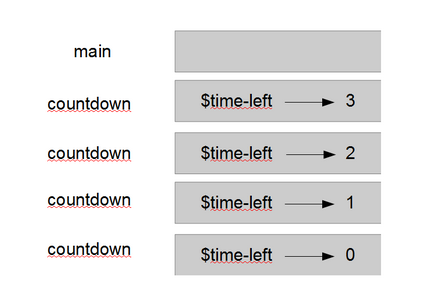
\includegraphics[scale=0.6]{figs/stack2.png}}
\caption{Stack diagram.}
\label{fig.stack2}
\end{figure}


As usual, the top of the stack is the frame for the main 
program.
It is empty because we did not create any variables in 
it or pass any arguments to it.
\index{base case}
\index{recursion!base case}

The four {\tt countdown} frames have different values for the
parameter {\tt \$time-left}.  The bottom of the stack, where {\tt \$time-left = 0}, is
called the {\bf base case}.  It does not make a recursive call, so
there are no more frames.

As an exercise, draw a stack diagram for \verb"print-n-times" 
called with
\verb"$sentence = 'Hello'" and {\tt \$n = 2}.
Then write a function called \verb"do-n-times" that takes a function
and a number, {\tt \$num}, as arguments, and that calls
the given function {\tt \$num} times.
\label{do_n_times}

Solution: see Section~\ref{sol_do_n_times}


\section{Infinite Recursion}
\index{infinite recursion}
\index{recursion!infinite}
\index{runtime error}


If a recursion never reaches a base case, it goes on making
recursive calls forever, and the program never terminates.  This is
known as {\bf infinite recursion}, and it is generally not
a good idea. In fact, your program will not actually execute 
forever but will die at some point when the computer runs out of 
memory or some other critical resource.

You have to be careful when writing recursive subroutines. 
Make sure that you have a base case, and make sure that 
you are guaranteed to reach it. Actually, although this is not 
absolutely required by the language, I would advise you to 
take the good habit of treating the base case first.


\section{Keyboard Input}
\index{keyboard input}

The programs we have written so far accept no input from 
the user. They just do the same thing every time. Raku 
provides built-in functions that stop the program and
wait for the user to type something. 

For example, the {\tt prompt} function prompts the user with 
a question or an instruction. When the user presses 
{\sf Return} or {\sf Enter}, the program resumes and 
\verb"prompt" returns what the user typed as a string 
(without the newline character corresponding to the 
{\sf Return} key typed by the user):
\index{prompt function}
\index{function!prompt}

\begin{verbatim}
my $user = prompt "Please type in your name: ";
say "Hello $user";
\end{verbatim}
%

This is probably one of the most common ways to obtain 
interactive user input, because it is usually a good idea 
to tell the user what is expected.

Another possibility is to use the {\tt get} method (which
 reads a single line) on standard input:
\index{get function}
\index{function!get}

\begin{verbatim}
say "Please type in your name: ";
my $user = $*IN.get;
say "Hello $user";
\end{verbatim}
%
or the {\tt get} function, which reads a line from standard 
input by default:
\begin{verbatim}
say "Please type in your name: ";
my $user = get;
say "Hello $user";
\end{verbatim}
%

\section{Program Arguments and the MAIN Subroutine}
\label{MAIN}
\index{MAIN}

There is another (and often better) way to have a program 
use varying input defined by the user, which is to pass 
command-line arguments to the program, just as we have 
passed arguments to our subroutines.

The easiest way to retrieve arguments passed to a program is 
to use a special subroutine named \verb'MAIN'. A program that 
has a defined \verb'MAIN' subroutine will call automatically  
that subroutine and the command-line arguments supplied 
to the program will be passed as arguments to \verb'MAIN'. 
The \verb'MAIN' signature will enable you to 
retrieve the arguments provided in the command line and 
possibly also check their validity.
\index{signature}

For example, the {\tt greet.pl6} program might look like 
this:
\begin{verbatim}
sub MAIN (Str $name) {
    say "Hello $name";
}
\end{verbatim}

You may call this program twice with different command-line 
arguments as follows:

\begin{verbatim}
$ raku greet.pl6 Larry
Hello Larry

$ raku greet.pl6 world
Hello world
\end{verbatim}

It is very easy to change the argument, since all you need 
to do at the operating system command line is use the up arrow 
and edit the end of the previous command line.

If you forget to supply the argument (or provide the wrong 
number of arguments, or arguments not matching the signature), 
the program will die and Raku will nicely generate and 
display a usage method:

\begin{verbatim}
$ raku greet.pl6
Usage:
  greet.pl6 <name>
\end{verbatim}


\section{Debugging}
\label{whitespace}
\index{debugging}
\index{traceback}

When a syntax or runtime error occurs, the error message contains
a lot of information, but it can be overwhelming.  The most
useful parts are usually:

\begin{itemize}

\item What kind of error it was

\item Where it occurred

\end{itemize}

Syntax errors are usually easy to find, but there are a few
gotchas. In general, error messages indicate where the problem 
was discovered, but the actual error might be earlier in 
the code, sometimes on a previous line or even many lines 
before.
\index{multiplication tables}

For example, the goal of the following code was to display the 
multiplication tables:

\begin{verbatim}
# WARNING: faulty code
sub multiplication-tables {
    for 1..10 -> $x {
        for 1..10 -> $y {
            say "$x x $y\t= ", $x * $y;
        say "";
    }
}

multiplication-tables();
\end{verbatim}

It failed at compilation with the following error:

\begin{verbatim}
$ raku mult_table.pl6
===SORRY!=== Error while compiling /home/Laurent/mult_table.pl6
Missing block (taken by some undeclared routine?)
at /home/Laurent/mult_table.pl6:9
------> multiplication-tables();<HERE><EOL>
\end{verbatim}

The error message reports an error on line~9 of the program 
(the last line of the code), at the end of the line, but 
the actual error is a missing closing brace after line~4 
and before line~5. The reason for this is that, while the 
programmer made the mistake on line~4, the Raku interpreter 
could not detect this error before it reached the 
end of the program. The correct program for displaying 
multiplication tables might be:

\begin{verbatim}
sub multiplication-tables {
    for 1..10 -> $x {
        for 1..10 -> $y {
            say "$x x $y\t= ", $x * $y;
        }
        say "";
    }
}
multiplication-tables();
\end{verbatim}

When an error is reported on the last line of a program, 
it is quite commonly due to a missing closing parenthesis, 
bracket, brace, or quotation mark several lines earlier. 
An editor with syntax highlighting can sometimes help you.
\index{syntax!highlighting}

\index{error!runtime}
\index{runtime error}

The same is true of runtime errors. Consider this program 
aimed at computing 360 degrees divided successively by 
the integers between 2 and 5:

\begin{verbatim}
# WARNING: faulty code
my ($a, $b, $c, $d) = 2, 3, 5;
my $value = 360;
$value /= $_ for $a, $b, $c, $d;
say $value;
\end{verbatim}

This programs compiles correctly but displays a warning and 
then an exception on runtime:

\begin{verbatim}
Use of uninitialized value of type Any in numeric context 
in block  at product.pl6 line 3
Attempt to divide 12 by zero using div
  in block <unit> at product.pl6 line 4
\end{verbatim}
%

The error message indicates a ``division by zero'' exception 
on line~4, but there is nothing wrong with that line. 
The warning on line~3 might give us a clue that the 
script attempts to use an undefined value, but the real error 
is on the first line of the script, where one of the four 
necessary integers (4) was omitted by mistake from the list 
assignment.

\index{division by zero}
\index{uninitialized value}

You should take the time to read error messages carefully, 
but don't assume they point to the root cause of the 
exception; they often point to subsequent problems.


\section{Glossary}

\begin{description}

\item[Integer division] An operation, denoted {\tt div}, 
that divides two numbers and rounds down (toward zero) the 
result to an integer.
  \index{integer division} 
  \index{division!integer}

\item[Modulo operator]  An operator, denoted with a percent sign
({\tt \%}), that works on integers and returns the remainder when one
number is divided by another.
\index{modulo operator}
\index{operator!modulo}

\item[Boolean expression]  An expression whose value is either 
{\tt True} or {\tt False}.
\index{Boolean expression}
\index{expression!Boolean}

\item[Relational operator] One of the operators that compares
its operands. The most common numeric relational operators are 
{\tt ==}, {\tt !=}, {\tt >}, {\tt <}, {\tt >=}, and {\tt <=}. 
The equivalent string relational operators are {\tt eq}, {\tt ne}, 
{\tt gt}, {\tt lt}, {\tt ge}, and {\tt le}.

\item[Logical operator] One of the operators that combines Boolean
expressions: {\tt and}, {\tt or}, and {\tt not}. The equivalent 
higher-precedence operators are {\tt \&\&}, {\tt ||}, and {\tt !}

\item[Conditional statement]  A statement that controls the 
flow of execution depending on some condition.
\index{conditional!statement}
\index{statement!conditional}

\item[Condition] The boolean expression in a conditional 
statement that determines which branch runs.
\index{condition}

\item[Branch] One of the alternative sequences of statements in
a conditional statement.
\index{branch}

\item[Chained conditional]  A conditional statement with a 
series of alternative branches.
\index{chained conditional}
\index{conditional!chained}

\item[Nested conditional]  A conditional statement that appears
in one of the branches of another conditional statement.
\index{nested conditional}
\index{conditional!nested}

\item[Statement modifier] A postfix conditional expression, i.e., 
a conditional expression (using for example {\tt if}, {\tt unless} or 
{\tt for}) that is placed after the statement the executions of which 
it controls. It can also refer to a postfix looping expression.
\index{statement modifier}

\item[Return statement] A statement that causes a function to
end immediately and return to the caller.

\item[Recursion]  The process of calling the function that is
currently executing.
\index{recursion}

\item[Base case]  A conditional branch in a
recursive function that does not make a recursive call.
\index{base case}

\item[Infinite recursion]  A recursion that doesn't have a
base case, or never reaches it.  Eventually, an infinite 
recursion causes a runtime error, for which you may not want 
to wait because it may take a long time.
\index{infinite recursion}

\end{description}

\section{Exercises}
%

\begin{exercise}
%
Using the integer division and the modulo operators:
\index{modulo operator}
\index{operator!mod}
\index{mod, modulo operator}
\index{integer division}
\index{operator!div}
\index{div operator}
\label{int_div_modulo}

\begin{enumerate}

\item Write a subroutine that computes how many days, hours, minutes and seconds there are in the number of seconds passed as an argument to the subroutine.

\item Write a script that computes how many days, hours, minutes and seconds there are in 240,000 seconds.

\item Change your script to compute the number of days, hours, minutes and seconds there are in a number of seconds entered by the script user when prompted to give a number of seconds.

\end{enumerate}

Solutions: Subsection~\ref{sol_int_div_modulo}.

\end{exercise}


\begin{exercise}
\index{Fermat's Last Theorem}
\label{fermat_ex}

Fermat's Last Theorem says that there are no positive integers
$a$, $b$, and $c$ such that

\[ a^n + b^n = c^n \]
%
for any values of $n$ greater than 2.

\begin{enumerate}

\item Write a function named \verb"check-fermat" that takes four
parameters---{\tt a}, {\tt b}, {\tt c}, and {\tt n}---and
checks to see if Fermat's theorem holds.  If
$n$ is greater than 2 and 

\[a^n + b^n = c^n \]
%
the program should print, ``Holy smokes, Fermat was wrong!''
Otherwise the program should print, ``No, that doesn't work.''

\item Write a function that prompts the user to input values
for {\tt a}, {\tt b}, {\tt c}, and {\tt n}, converts them to
integers, and uses \verb"check-fermat" to check whether they
violate Fermat's theorem.
\end{enumerate}

Solution: \ref{sol_fermat_ex}


\end{exercise}


\begin{exercise}
\index{triangle}
\label{triangle}

If you are given three sticks, you may or may not be able to arrange
them in a triangle.  For example, if one of the sticks is 12 inches
long and the other two are one inch long, you will
not be able to get the short sticks to meet in the middle.  For any
three lengths, there is a simple test to see if it is possible 
to form a triangle:

\begin{quotation}
If any of the three lengths is greater than the sum of the other
  two, then you cannot form a triangle.  Otherwise, you
  can.  (If the sum of two lengths equals the third, they form
    what is called a ``degenerate'' triangle.)
\end{quotation}

\begin{enumerate}

\item Write a function named \verb"is-triangle" that takes three
positive numbers as arguments, and that prints either 
``Yes'' or ``No,'' depending on whether you can 
form a triangle from sticks with the given lengths.

\item Write a function that prompts the user to input 
three stick lengths and uses \verb"is-triangle" to check 
whether sticks with the given lengths can form a triangle.

\end{enumerate}

Solution: \ref{sol_triangle}


\end{exercise}

\begin{exercise} 
\index{Fibonacci!numbers}
\label{fibonacci}
The Fibonacci numbers were invented by Leonardo Fibonacci 
(a.k.a. Leonardo of Pisa or simply Fibonacci), an Italian 
mathematician of the thirteenth century.
\index{Fibonacci, Leonardo}

The Fibonacci numbers are a sequence of numbers such as:

\[1, \;1, \;2, \;3, \;5, \;8, \;13, \;21, \;34, \ldots\]
%
in which the first two numbers are equal to 1 and each 
subsequent number of the sequence is defined as the sum of 
the previous two (for example, $5 = 2 + 3$, $8 = 3 + 5$, etc.).

In mathematical notation, the Fibonacci numbers could be defined by recurrence as follows:

\[F_1 = 1, \;F_2 = 1, \;\;and\;\;  F_n = F_{n-1} + F_{n-2} \]
%
\begin{enumerate}

\item Write a program using a {\tt for} loop that prints on screen the first 20 Fibonacci numbers.

\item Write a program which prompts the user to enter a number 
$n$ and, using a {\tt for} loop, computes and displays the 
$n^{th}$ Fibonacci number.

\end{enumerate}

Solution: \ref{sol_fibonacci}


\end{exercise}

\begin{exercise}
\label{sub_recurse}
\index{recursion}

What is the output of the following program?
Draw a stack diagram that shows the state of the program
when it prints the result.

\begin{verbatim}[fontshape=up]
sub recurse($n, $s) {
    if ($n == 0) {
        say $s;
    } else {
        recurse $n - 1, $n + $s;
    }
}
recurse 3, 0;
\end{verbatim}

\begin{enumerate}

\item What would happen if you called the function like 
this: {\tt recurse(-1, 0)}?

\item Write a documentation comment (maybe in the form of a multiline comment) that explains everything someone would need to know in order to use this function (and nothing else).

\end{enumerate}

Solution: \ref{sol_sub_recurse}

\end{exercise}


